
\documentclass[
   ngerman          % neue deutsche Rechtschreibung
  ,a4paper          % Papiergrösse
% ,twoside          % Zweiseitiger Druck (rechts/links)
% ,10pt             % Schriftgrösse
  ,11pt
% ,12pt
  ,pdftex
%  ,disable         % Todo-Markierungen auschalten
]{report}

\usepackage[utf8]{inputenc}        

\usepackage{dokumentation}

%% ACHTUNG, wenn man eine eigene Formatdatei (bericht.fmt) benutzt, werden Änderungen an bericht.sty
%% erst wirksam, wenn die Format-Datei neu erzeugt wurde!!!
%% Genauer alle Änderungen, die textuell vor der nächsten Zeile ".... endofdump...." stehen
%% werden erst wirksam, wenn die Formatdatei neu erzeugt wurde
\csname endofdump\endcsname

%%%%%%%%%%%%%%%%%%%%%%%%%%%%%%%%%%%%%%%%%%%%%%%%%%%%%%%%%%%%%%%%%%%%%%%%%%%%%%%
%% Angaben zur Arbeit
%%%%%%%%%%%%%%%%%%%%%%%%%%%%%%%%%%%%%%%%%%%%%%%%%%%%%%%%%%%%%%%%%%%%%%%%%%%%%%%

\newcommand{\Autor}{Toni Einecker}
\newcommand{\MatrikelNummer}{3523850}
\newcommand{\Kursbezeichnung}{Tinf18B3}
\newcommand{\FirmenName}{SICK AG}
\newcommand{\FirmenStadt}{Waldkirch}
\newcommand{\DhbwLogoDeckblatt}{
\includegraphics[width=4cm]{Bilder/dhbwLogo.PNG}}

%%%%%%%%%%%%%%%%%%%%%%%%%%%%%%%%%%%%%%%%%%%%%%%%%%%%%%%%%%%%%%%%%%%%%%%%%%%%%%

\newcommand{\Titel}{Dokumentation des Projekts}
\newcommand{\Was}{Wortfinder}
\newcommand{\AbgabeDatum}{17. Mai 2021}
\newcommand{\Abschluss}{Bachelor of Science}
\newcommand{\Studiengang}{Informatik / Informationstechnik}

\hypersetup{%%
  pdfauthor={\Autor},
  pdftitle={\Titel},
  pdfsubject={\Was}
}

%%%%%%%%%%%%%%%%%%%%%%%%%%%%%%%%%%%%%%%%%%%%%%%%%%%%%%%%%%%%%%%%%%%%%%%%%%%%%%%

\includeonly{
 einleitung,
 unitTests,
 cleanArchitecture,
 codeSmells,
 entwurfsmuster,
 programmingPrinciples,
 anhang
}
%%%%%%%%%%%%%%%%%%%%%%%%%%%%%%%%%%%%%%%%%%%%%%%%%%%%%%%%%%%%%%%%%%%%%%%%%%%%%%%
%% Titelseite
%%%%%%%%%%%%%%%%%%%%%%%%%%%%%%%%%%%%%%%%%%%%%%%%%%%%%%%%%%%%%%%%%%%%%%%%%%%%%%%

\begin{document}
\begin{titlepage}
\begin{center}
\vspace*{-2cm}
%\FirmenLogoDeckblatt
\hfill\DhbwLogoDeckblatt\\[2cm]
{\Huge \Titel}\\[1cm]
{\Huge\scshape \Was}\\[1cm]
{\large für die Prüfung zum}\\[0.5cm]
{\Large \Abschluss}\\[0.5cm]
{\large des Studienganges \Studiengang}\\[0.5cm]
{\large an der}\\[0.5cm]
{\large Dualen Hochschule Baden-Württemberg Karlsruhe}\\[0.5cm]
{\large von}\\[0.5cm]
{\large\bfseries \Autor}\\[1cm]
{\large Abgabedatum \AbgabeDatum}
\vfill
\end{center}
\begin{tabular}{l@{\hspace{2cm}}l}
Matrikelnummer	                 & \MatrikelNummer		\\
Kurs			         & \Kursbezeichnung		\\
\end{tabular}
\end{titlepage}

%%%%%%%%%%%%%%%%%%%%%%%%%%%%%%%%%%%%%%%%%%%%%%%%%%%%%%%%%%%%%%%%%%%%%%%%%%%%%%%
%% Verzeichnisse
%%%%%%%%%%%%%%%%%%%%%%%%%%%%%%%%%%%%%%%%%%%%%%%%%%%%%%%%%%%%%%%%%%%%%%%%%%%%%%%

\pagenumbering{Roman}
\newpage
\tableofcontents

%%%%%%%%%%%%%%%%%%%%%%%%%%%%%%%%%%%%%%%%%%%%%%%%%%%%%%%%%%%%%%%%%%%%%%%%%%%%%%%
%% Inhalt
%%%%%%%%%%%%%%%%%%%%%%%%%%%%%%%%%%%%%%%%%%%%%%%%%%%%%%%%%%%%%%%%%%%%%%%%%%%%%%%
\cleardoublepage
\setcounter{savepage}{\arabic{page}}
\pagenumbering{arabic}
\chapter{Einleitung}

Die Anwendung \glqq Wortfinder\grqq{} ist ein Spiel, welches dem Spielprinzip von Wortopia nachempfunden ist. Im Gegensatz zu Wortopia ist diese Anwendung allerdings vollständig offline verfügbar.

%% Spiel prinzip
Das Spielprinzip ist sehr Simpel. Es wird ein Raster mit Buchstaben angezeigt und in diesem müssen in einer vorgegebenen Zeit möglichst viele Wörter gefunden werden. Zum finden der Wörter lassen sich die Buchstaben mit der Maus verbinden. Je nach Länge des Wortes und der initialen Spielzeit, gibt es für jedes Wort Punkte. Nach einer Partie kann der Spieler seinen Highscore speichern. Die Highscores werden dabei nur lokal gespeichert.


%% Funktionalität
\paragraph{Grobe Funktionalität}
Die Buchstabenraster werden als \glqq Game\grqq{} Objekte verwaltet. In diesen befindet sich neben dem Buchstabenraster, auch eine Liste aller korrekten findbaren Wörter. Somit kann beim laufenden Spiel angezeigt werden, wie viele Wörter insgesamt findbar sind. Dafür werden diese Objekte im Vorhinein generiert und gespeichert. Dadurch kann direkt nach dem Start der Anwendung mit dem Spielen begonnen werden und es muss nicht auf das fertige generieren von Feldern gewartet werden.

\paragraph{Repositories}
Der Quellcode der Anwendung sowie die Unit Tests befinden sich in folgendem Repository:
\begin{itemize}
\item \textbf{Quellcode:} \href{https://github.com/EinToni/Wortfinder}{github.com/EinToni/Wortfinder}
\end{itemize}

Nachfolgend sind noch die direkten Links zum Anwendungscode sowie zu den Tests aufgelistet. Außerdem ist auch das Repository mit dieser Dokumentation verlinkt, damit unter Umständen manche Bilder im Original und vergrößert betrachtet werden können.

\begin{itemize}
\item \textbf{Anwendungscode:} \href{https://github.com/EinToni/Wortfinder/tree/main/Wortfinder}{github.com/EinToni/Wortfinder/tree/main/Wortfinder}
\item \textbf{Unit Tests:} \href{https://github.com/EinToni/Wortfinder/tree/main/Wortfinder.XUnitTests}{github.com/EinToni/Wortfinder/tree/main/Wortfinder.XUnitTests}
\item \textbf{Dokumentation:} \href{https://github.com/EinToni/WortfinderDoku}{github.com/EinToni/WortfinderDoku}
\end{itemize}

\chapter{Unit Tests}

Bei der Erstellung der Tests wurde stets versucht auf die ATRIP-Regeln zu beachten. Die einzelnen Punkte sind im folgenden genauer aufgeführt.

\paragraph{Automatic}
Damit die Tests eigenständig ablaufen und ihre Ergebnisse selbst überprüfen, wird xUnit verwendet. D.h. die Tests werden als \glqq Fact\grqq{} annotiert und können dann automatisch ausgeführt werden. Es sind keine Benutzereingaben bei den Tests erforderlich und sie liefern immer das Ergebnis \glqq bestanden\grqq{} oder \glqq nicht bestanden\grqq{}.

\paragraph{Thorough}
Der Fokus wurde darauf gelegt das Wichtigste zu testen. Allerdings sind auch manche weniger relevanten Klassen abgedeckt, welche sich einfach Testen lassen und die Test Erstellung daher schnell ging. Ein Beispiel dafür ist der \href{https://github.com/EinToni/Wortfinder/blob/main/Wortfinder/GameScore.cs}{\textit{GameScore}}, welcher die Punkte des aktuellen Spiels zählt, somit nicht Missions-kritisch ist, aber dennoch abgedeckt wurde. Es wurde allerdings auch nicht jede wichtige Funktionalität getestet. Beispiele hierfür sind die GUI Elemente, welche nicht mit Tests abgedeckt sind.
%% Mehrere Szenarien abgedeckt

\paragraph{Repeatable}
Durch die Nutzung von xUnit lassen sich die Tests jederzeit auf Knopfdruck automatisch ausführen. Die Ergebnisse haben bis Dato immer das gleiche Ergebnis geliefert und sollten dies auch weiterhin, da keine direkten Festplattenzugriffe oder zeitabhängige Funktionen getestet wurden. 

\paragraph{Independent}
Die Tests sind unabhängig voneinander. Außerdem werden sie durch xUnit in einer unbekannten und nicht vorhersagbaren Reihenfolge ausgeführt.

\paragraph{Professional}
Es wurde versucht den Testcode möglichst einfach, leserlich und kurz zu halten. Für das bessere Verständnis wurden meistens erklärende Variablen eingeführt, anstelle die Werte direkt zu verwenden. Allerdings wurde im Nachhinein festgestellt, dass dies nicht immer eingehalten wurde. Vor allem bei sehr kurzen Tests wurde auf extra Variablen verzichtet. In der folgenden Abbildung sieht man links einen einfach verständlichen Test mit extra Variablen und rechts einen Test ohne extra Variablen, welcher dafür aufgrund der Kürze immer noch recht verständlich ist.

\begin{figure}[!htb]
\centering
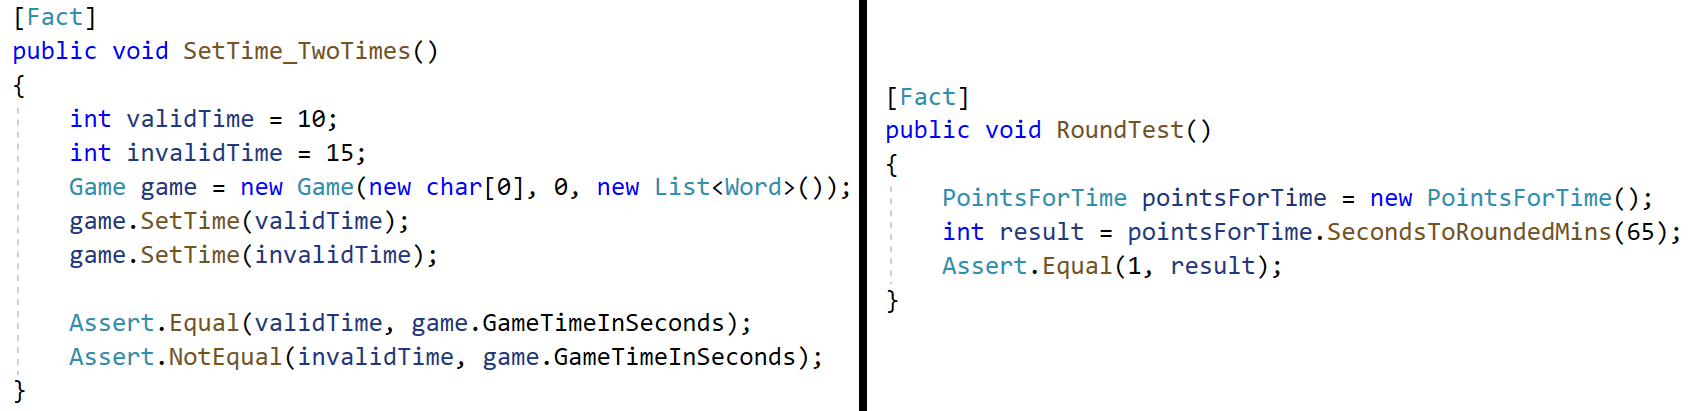
\includegraphics[width=0.95\textwidth]{Bilder/professional_example.PNG}
\caption{\label{Abb:professional_example} Professional Beispiel in ATRIP}
\end{figure}


\paragraph{Struktur}
Die Tests wurden in der AAA-Normalform erstellt. Mock-Objekte wurden mit Moq erstellt. Ein Beispiel für die Normalform sowie die Verwendung von Mocks ist nachfolgend dargestellt. Dabei werden im \glqq Arrange\grqq{} Part 5 Mocks erstellt, da diese im Konstruktor der Klasse benötigt werden und anschließend eine Instanz der Klasse erzeugt. Die Mocks werden nicht weiter konfiguriert, da sie nur für die Dependency Injection im Konstruktor benötigt werden, aber nicht für den eigentlichen Test. Danach folgt der \glqq Act\grqq{} Part, d.h. die Ausführung, in welchem die zu testende Funktion aufgerufen wird. Abschließend folgt der \glqq Assert\grqq{} Teil, in welchem überprüft wird ob das Ergebnis korrekt ist.


In dem dargestellten Tests wird dabei überprüft ob die Variable \glqq GameRunning\grqq{}, welche angibt ob ein Spiel am laufen ist, nach dem stoppen des Spiels korrekt auf \glqq false\grqq{} gesetzt wurde.


\begin{figure}[!htb]
\centering
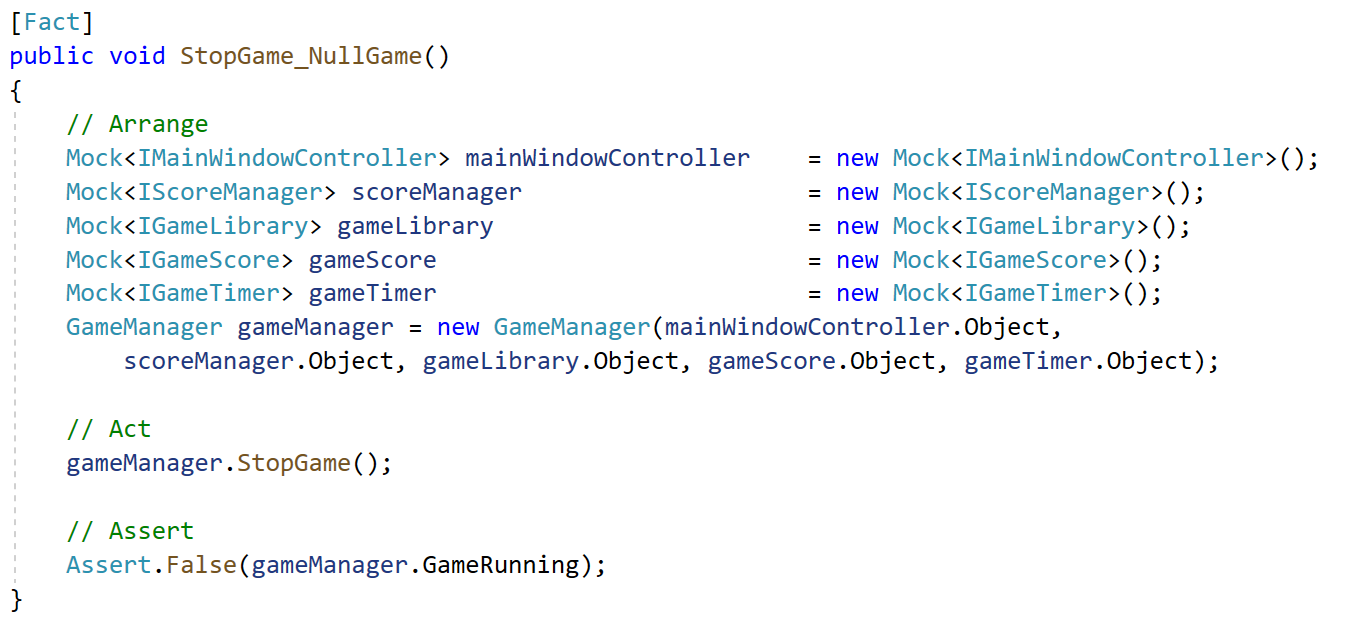
\includegraphics[width=0.95\textwidth]{Bilder/UnitTest.PNG}
\caption{\label{Abb:UnitTest}Beispiel Tests mit Mocks in AAA-Normalform}
\end{figure}

\newpage
\paragraph{Code-Coverage} Zur Bestimmung der Test Abdeckung wurde die diesbezügliche Funktionalität in Visual Studio Enterprise verwendet, welche aufgrund der Studenten Lizenz zur Verfügung steht. Die Testabdeckung der Anwendung beträgt ca. 50\% Line Coverage. Im nachfolgenden Ergebnisausschnitt dürfen dabei nur die Prozentangaben in der blau markierte Zeile beachtet werden, da dies das Projekt mit dem Anwendungscode ist.

\begin{figure}[!htb]
\centering
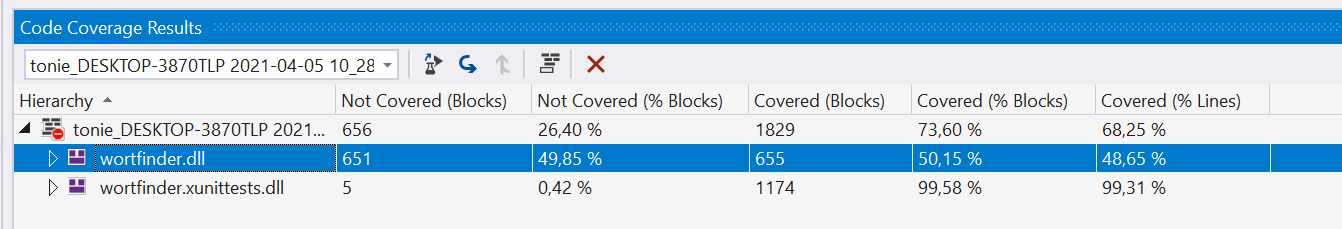
\includegraphics[width=0.95\textwidth]{Bilder/Testabdeckung.PNG}
\caption{\label{Abb:Testabdeckung}Die Ausgabe der Testabdeckung von Visual Studio}
\end{figure}

Die Abdeckung ist nicht höher, da ein großer Anteil der Codezeilen in den \textit{xaml} Dateien der GUI sind, welche nicht abgedeckt und nicht Unit Testbar sind. Außerdem sind wie schon erwähnt primär die wichtigen Stellen im Quellcode mit Tests abgedeckt. Unwichtigere werden eher vernachlässigt. Die Abdeckung könnte somit noch erhöht werden, wäre aber mit viel Aufwand verbunden welcher hier als nicht vertretbar angesehen wird.

\endinput
\chapter{Clean Architecture}\label{cleanArchitecture}

Zum implementieren der Clean Architecture wurde ein UML Diagramm erstellt (Abb.~\ref{Abb:CleanArchitectureBEFORE} im Anhang) um die aktuellen Abhängigkeiten zu sehen, dabei wurden ein paar Abhängigkeitspfeile weggelassen welche von weit außen nach innen gehen und die Lesbarkeit zu sehr verringern. 


Für die Struktur der Clean Architektur wurde sich auf 4 Schichten festgelegt, da die Funktionsweise des Programms recht simpel ist. Die innerste Schicht beinhaltet alle Entitäten welche zur strukturierten Datenspeicherung verwendet werden. Die mittlere hellblaue Schicht umfasst die Anwendungslogik. Die dunkelgrüne Schicht beinhaltet die Interaktion mit allem Außerhalb, d.h. die Controller zum lesen und schreiben der Daten auf der Festplatte sowie zum kommunizieren mit der GUI. Ganz außen befinden sich die Speicherorte der Spieldaten und die GUI Elemente. 


\begin{figure}[!ht]
  \centering
  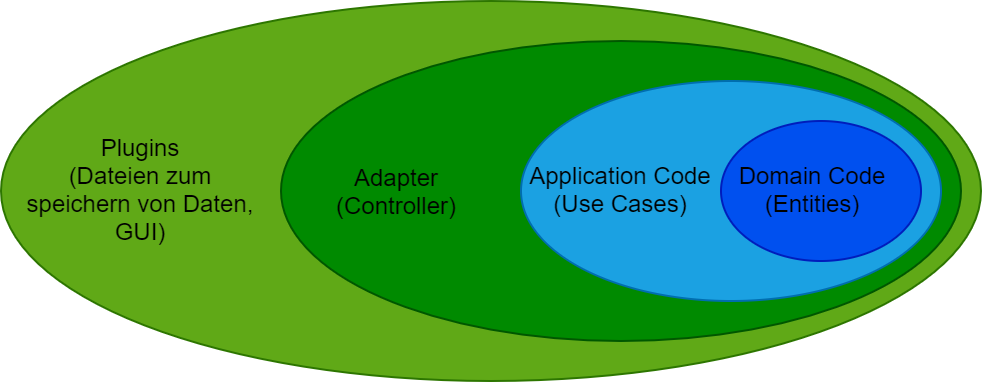
\includegraphics[width=0.6\textwidth]{Bilder/ArchitekturSchichten.PNG}
  \caption{Aufbau der Schichten der Clean Architecture in der Anwendung}
  \label{Abb:ArchitekturSchichten}
\end{figure}

\paragraph{Abhängigkeiten}
Ein großes Problem sind die Abhängigkeiten von Innen nach Außen, wie z.B. die \href{https://github.com/EinToni/Wortfinder/blob/main/Wortfinder/WordGenerator.cs}{\textit{WordFinder}} (umbenannt zu \textit{WordGenerator}) Klasse, welche direkt auf den \href{https://github.com/EinToni/Wortfinder/blob/586681478211a26abc661239ecc2c297ef77041e/Wortfinder/DataController.cs}{\textit{DataController}} zugreift, siehe.~\ref{Abb:CleanArchitectureBEFORE} auf Seite~\pageref{Abb:CleanArchitectureBEFORE}. Die Abhängigkeit wird durch Dependency Inversion, d.h. die Erstellung eines Interfaces welches von der äußeren Klasse implementiert und von der inneren genutzt wird, umgedreht. Die Dependency Inversion ist in der nachfolgenden Abbildung dargestellt und in Commit \href{https://github.com/EinToni/Wortfinder/commit/586681478211a26abc661239ecc2c297ef77041e}{586681478211a26abc661239ecc2c297ef77041e} umgesetzt.
\newpage
\begin{figure}[!ht]
  \centering
  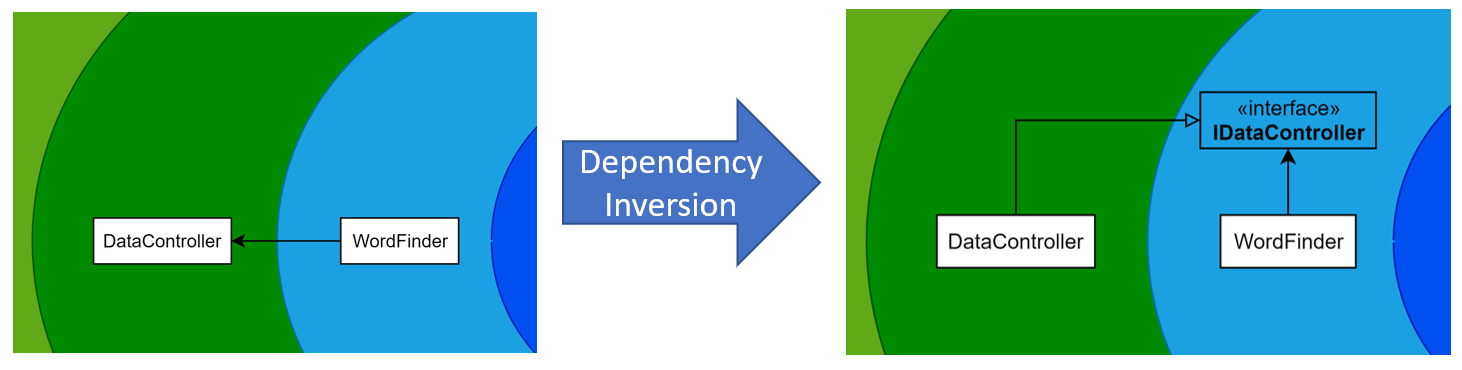
\includegraphics[width=0.8\textwidth]{Bilder/DependencyInversion.PNG}
  \caption{Beispiel der Dependency Inversion}
  \label{Abb:DependencyInversion}
\end{figure}

\paragraph{Abstrakte Fabrik}
Oftmals haben Klassen in inneren Schichten, Klassen aus äußeren Schichten instantiiert. Ein Beispiel dafür ist ebenfalls der  \textit{WordFinder}, welcher im Konstruktor eine eine Instanz des \textit{DataController} erstellt hat. Unter Einhaltung der Clean Architecture geht das allerdings nicht. Da vermieden werden wollte, dass die Referenzen auf diese äußeren Klassen von der Main aus weit \glqq nach unten gereicht\grqq{} werden, wurde das Erzeugungsmuster der abstrakten Fabrik verwendet. Dem \textit{WordFinder} wird dann im Konstruktor eine Referenz auf die Fabrik gegeben. Über die Funktion \glqq GetDataController()\grqq{} gibt die Fabrik dann eine neue Instanz des \textit{DataController} zurück, wobei der Rückgabetyp im Interface der Fabrik als \textit{IDataController} Deklariert ist, vgl. Commit \href{https://github.com/EinToni/Wortfinder/commit/26148d6a7ae6784b935a260371672fe16f8bbfa0}{26148d6a7ae6784b935a260371672fe16f8bbfa0}:

\begin{figure}[!ht]
  \centering
  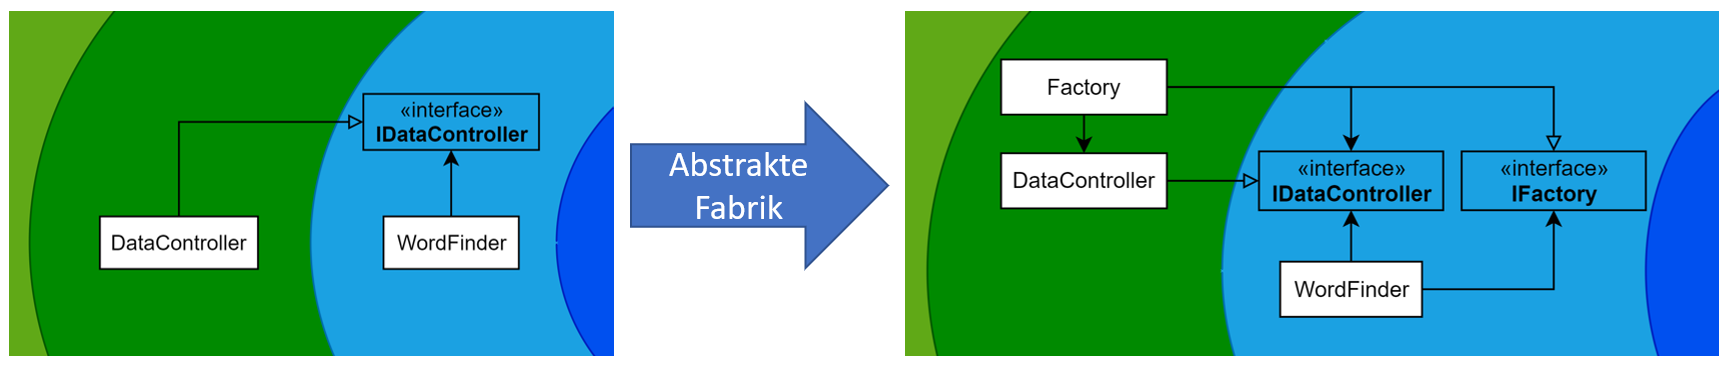
\includegraphics[width=0.8\textwidth]{Bilder/AbstrakteFabrik.PNG}
  \caption{Implementierung der abstrakten Fabrik}
  \label{Abb:AbstrakteFabrik}
\end{figure}

\paragraph{Separierung der GUI}
Außerdem problematisch ist der grundsätzliche Aufbau des Programms, sowie speziell der Aufbau des Hauptfensters. Dieses bestand aus einem Grid welches durch den \textit{FieldGenerator} mit Teilfenstern (\textit{LetterBox}, zeigen die Buchstaben an) gefüllt wurde. Jeder \textit{LetterBox} wurde die Instanz des \textit{WordBuilder} gegeben, welchen sie aufrufen wenn sie angeklickt werden.


Zur Verbesserung der Trennung zwischen dem Application Code und der GUI, wird das Grid direkt im Code Behind des \textit{MainWindow} mit WPF  Elementen aufgebaut. Die Ansteuerung des \textit{MainWindow} erfolgt dann über einen neuen \textit{MainWindowController} dem im Aufruf nur die Größe des Spielfelds und die Buchstaben übergeben werden. Somit erfolgt die Erstellung der GUI separiert vom restlichen Anwendungscode.

\paragraph{Umsetzung}
Vor der eigentlichen Implementierung wurde zuerst das erstellte UML Diagramm abgeändert. Zuerst wurde dabei die Struktur geändert, sodass alle Klassen an ihrem sinnvollsten Ort sind. Dann wurden alle Abhängigkeitspfeile welche nach außen zeigen mittels Dependency Inversion umgedreht und als letztes an notwendigen Stellen eine Abstrakte Fabrik hinzugefügt. 

Da die Anwendung vorher immer nur mit Funktionen ergänzt wurde und dabei lediglich Wert auf Funktionalität gelegt wurde, sind einige unnötig komplexe Strukturen entstanden. Diese wurde daher ebenfalls direkt geändert.
Ein Beispiel hierfür ist die \textit{FindableWords} Klasse, welche alle im aktuelle laufenden Spiel findbaren Wörter beinhaltet. Diese wurde erst später hinzugefügt, da davor direkt jedes vom Nutzer markierte Wort im heruntergeladenen Wörterbuch überprüft wurde. Sowie die \textit{GameGrid} Klasse, welche (unter anderem) die Größe und Buchstaben des Spielfelds beinhaltet. Die findbaren Wörter sowie die Buchstaben im aktuellen Spiel wurden in eine neue Klasse \textit{Game} verschoben welche alle Daten über Spiel enthält. Dies ermöglicht das generieren im Vorhinein anschließende und speichern von Spielen.

Das daraus entstandene Diagramm ist im Anhang als Abbildung~\ref{Abb:CleanArchitectureAFTER}.


\paragraph{Klassen Instantiierung}
Manche Klassenreferenzen werden trotz der Abstrakten Fabrik teilweise immer noch sehr weit an nachfolgende Klassen \glqq weitergereicht\grqq, was sehr unschön ist. Daher wurde die Erstellung aller Klassen und deren Dependency Injection in die Main verschoben. Dadurch wird das unschöne und unübersichtliche weiterreichen vermieden. Auch die Erzeugung von Klassen im Konstruktor wird durch Dependency Injection ersetzt, wodurch beim Testen ein Mock-Objekt an die zu testende Klasse übergeben werden kann. Außerdem können die abstrakten Fabriken hierdurch auch wieder entfernt werden, da alle Klassen direkt in der Main erzeugt werden und von den betroffenen Klassen nur eine Instanz benötigt wird. Der Commit in welchem alle Initialisierungen in die Main ausgelagert wurde und somit die Implementierung der Clean Architecture abgeschlossen ist, ist: \href{https://github.com/EinToni/Wortfinder/commit/15e467c93903dac44e916c61f76792d385abd087}{15e467c93903dac44e916c61f76792d385abd087}. Das sich hieraus ergebende Klassendiagramm ist im Anhang~\ref{Abb:CleanArchitectureAFTERinMain}.


\paragraph{Nachträgliche Korrektur}
Nicht eingehalten wurde die Clean Architecture bei der \textit{WebScraper} und \textit{WordMissingWindow} Klasse. Die beiden Klassen wurden dabei direkt aus dem Controller des \textit{MainWindow}s aufgerufen. Denn zum Zeitpunkt des Commits war geplant diese nicht mehr zu verwenden und später zu entfernen. Da sie allerdings in Zukunft doch noch verwendet werden sollen, wurden sie, sowie weitere zugehörige Klassen, im Nachhinein korrekt angepasst. Das Klassendiagramm nach welchem die Implementierung durchgeführt wurde ist nachfolgend abgebildet. Zu beachten ist allerdings, dass nur die Struktur und die GUI implementiert wurden. Für die korrekte Funktionalität des WebScrapers fehlte leider die Zeit. Diese soll aber in Zukunft online im Duden das als fehlend angegebene Wort nachschlagen und prüfen ob es existiert. Commit der Implementierung: \href{https://github.com/EinToni/Wortfinder/commit/163a14f0730bb69c9805b4ee0421e415ce8c897d}{163a14f0730bb69c9805b4ee0421e415ce8c897d}

\begin{figure}[htb]
\centering
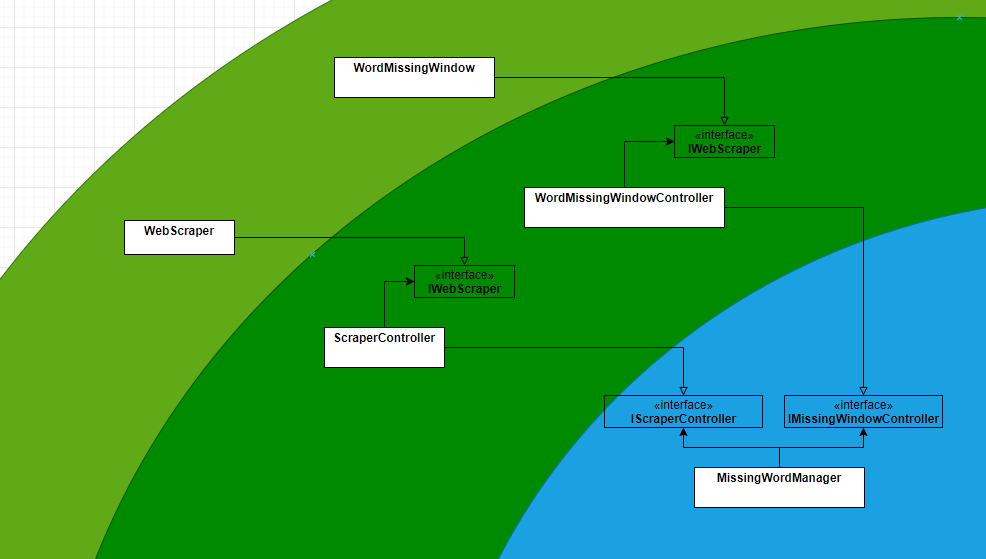
\includegraphics[width=0.8\textwidth]{Bilder/CleanArchitectureWebScraper.PNG}
\caption{\label{Abb:CleanArchitectureWebScraper}Vereinfachtes Klassendiagramm des WebScrapers und zugehöriger GUI}
\end{figure}

\endinput
\chapter{Code Smell Refactoring}

\subsection{Long Method}

Die Klasse \textit{WordGenerator} ist dafür zuständig alle möglichen Wörter in einem Raster von Buchstaben zu finden. Dafür hat sie zwei Funktionen welche jeweils ca. 50 Zeilen lang sind. Beide Funktionen sind durch viele Schleifen sehr unübersichtlich und fallen unter die Long Method Code Smells. Zum Refactoren des Code Smells wird die Funktion zuerst mittels Extract Method in kleinere Funktionen unterteilt. Dabei wurde direkt noch die If-Abfrage zur besseren Lesbarkeit umgedreht. Die extrahierten Methoden sind in Abb.~\ref{Abb:ExtractMethod} in Grün und Orange markiert. (Commit:~\href{https://github.com/EinToni/Wortfinder/commit/b6e3b31e4ef7b597863bc2be073f9e136d4b9594}{b6e3b31e4ef7b597863bc2be073f9e136d4b9594})

\begin{figure}[!ht]
  \centering
  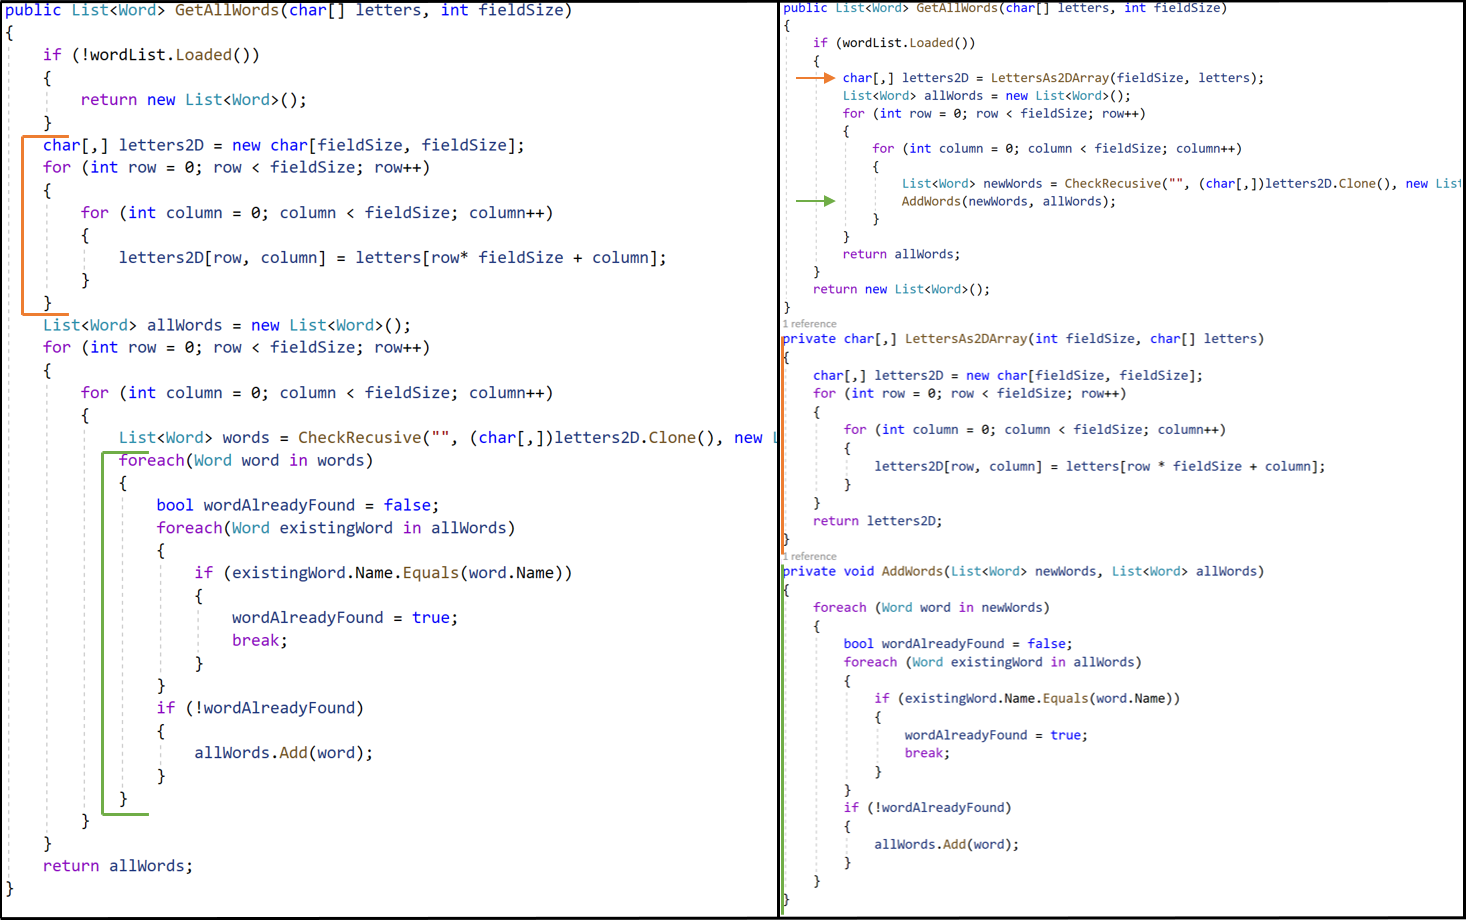
\includegraphics[width=\textwidth]{Bilder/ExtractMethod.PNG}
  \caption[Anwendung des Extract Method Refactoring]{Anwendung des Extract Method Refactoring (\href{https://github.com/EinToni/WortfinderDoku/blob/main/Bilder/ExtractMethod.png}{Link})}
  \label{Abb:ExtractMethod}
\end{figure}

Danach fallen die zwei gleichen Schachtelungen der for-Schleifen auf. Dabei wird in der Funktion \textit{LettersAs2DArray} das Array zu einem 2D Array umstrukturiert, da die Buchstaben in einen Raster angeordnet sind ist so ein Iterieren und suchen von Nachbarn einfacher vorstellbar. Da zwischenzeitlich allerdings die \textit{Coordinate} Klasse eingefügt wurde, welche das Prüfen auf Nachbarschaft übernimmt, lässt sich dieser Code vereinfachen. Das durchlaufen des 2D Arrays (Abb.~\ref{Abb:CodeVereinfachen} Orange markiert) wird somit durch ein einmaliges durchlaufen des Ursprünglichen Arrays ersetzt. Die \textit{LettersAs2DArray} Funktion wird hier nur noch für den Aufruf an die nächste Funktion benötigt und kann nach dessen Refactorings komplett entfernt werden. Außerdem kann die in Grün markierte Funktionalität, welche überprüft ob ein Wort schon in der List ist, ebenfalls durch Extract Method ausgelagert werden. Es ergibt sich somit folgender Code (Commit:~\href{https://github.com/EinToni/Wortfinder/commit/f733dabc6753529e597408cc8c76ea0a39a1ff8e}{f733dabc6753529e597408cc8c76ea0a39a1ff8e}):

\begin{figure}[!ht]
  \centering
  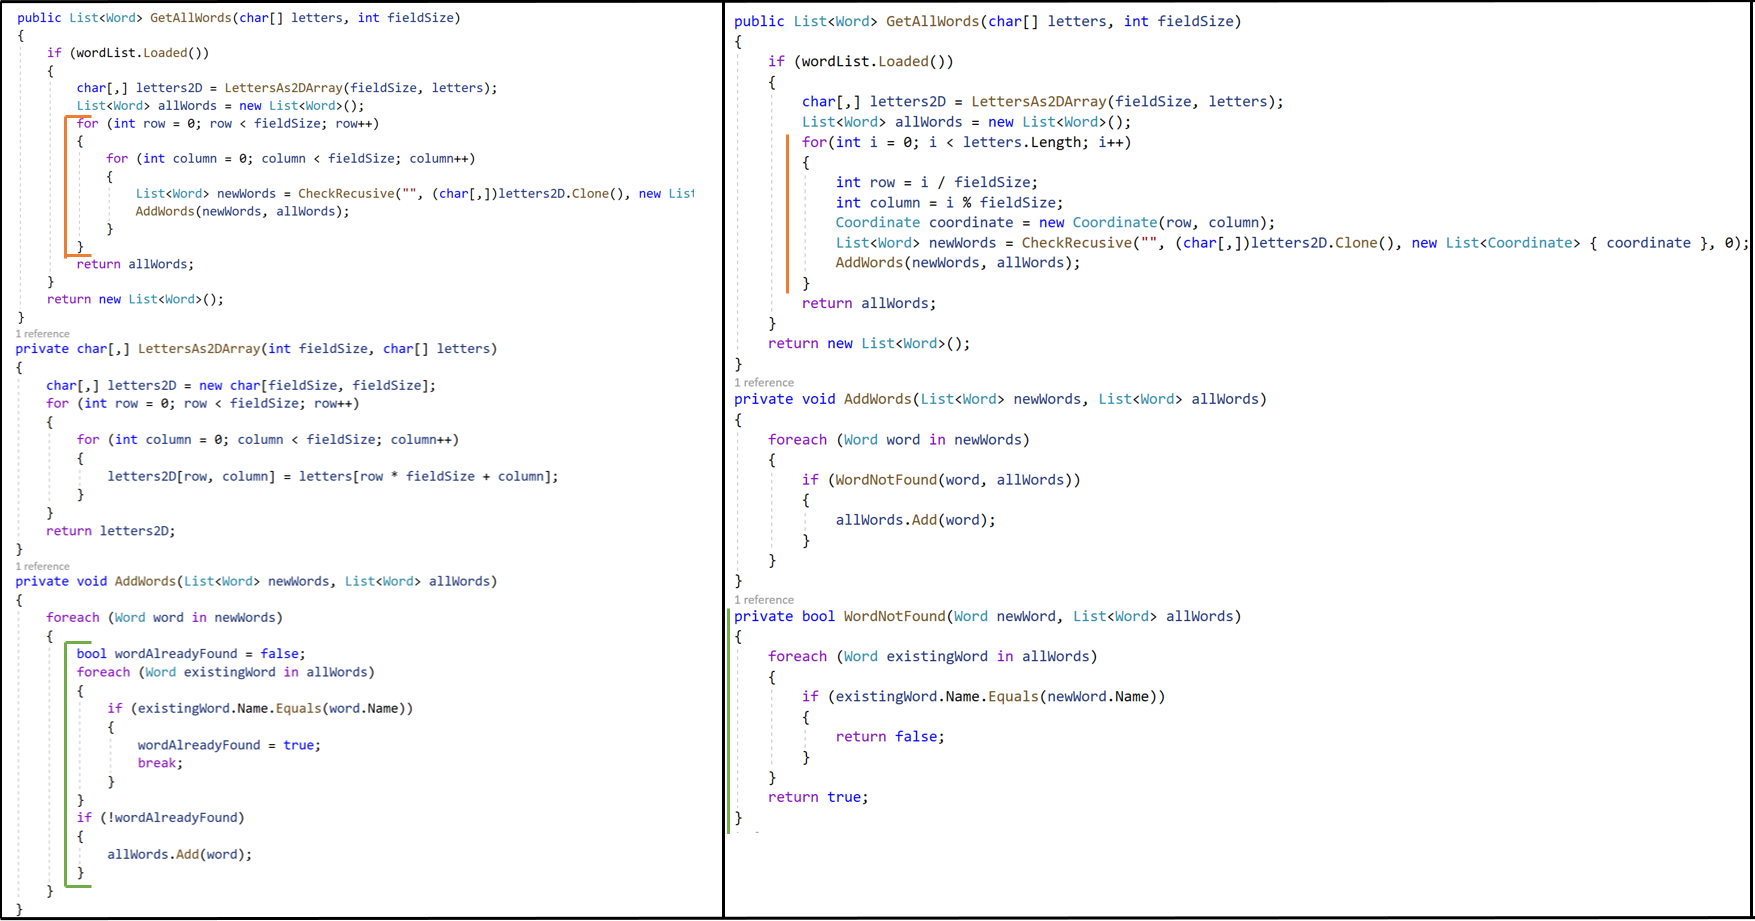
\includegraphics[width=\textwidth]{Bilder/CodeVereinfachen.PNG}
  \caption[Extract Method und Code Vereinfachung]{Extract Method und Code Vereinfachung (\href{https://github.com/EinToni/WortfinderDoku/blob/main/Bilder/CodeVereinfachen.png}{Link})}
  \label{Abb:CodeVereinfachen}
\end{figure}

In der zweiten Funktion wird ebenfalls mit Extract Method begonnen (Abb.~\ref{Abb:ExtractMethod2}). Dabei werden zwei verschachtelte Schleifen ausgelagert, in welchen die betroffene Methode Rekursiv wieder aufgerufen wird. Da bei der Rekursion alle Parameter mitgegeben werden müssen ist ein komplettes auslagern unvorteilhaft, da in diese neue Methode dann ebenfalls alle Parameter weitergegeben werden müssten. Daher wird nur der Teil in eine neue Methode verschoben (Orange markiert), welcher alle benachbarten Positionen im Buchstabengitter findet, Commit: \href{https://github.com/EinToni/Wortfinder/commit/23cf0b7d1165c1d17235d68f8fca35682ba233ad}{23cf0b7d1165c1d17235d68f8fca35682ba233ad}):
\newpage
\begin{figure}[!ht]
  \centering
  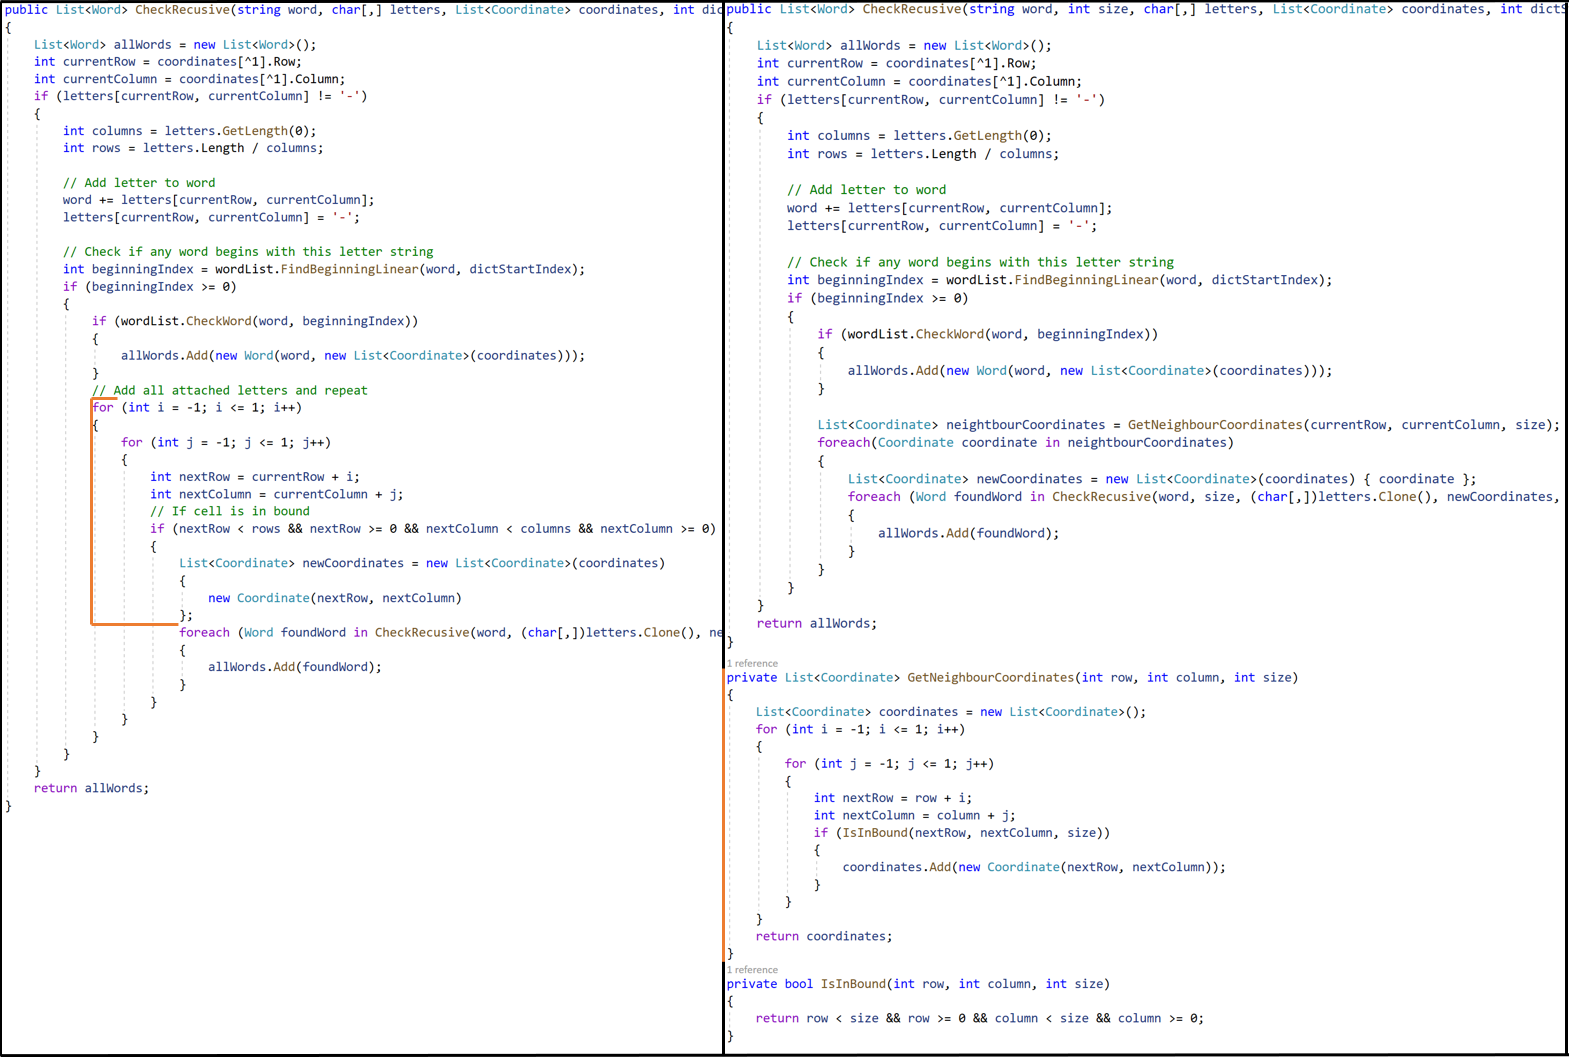
\includegraphics[width=\textwidth]{Bilder/ExtractMethod2.PNG}
  \caption[Extract Method]{Extract Method (\href{https://github.com/EinToni/WortfinderDoku/blob/main/Bilder/ExtractMethod2.png}{Link})}
  \label{Abb:ExtractMethod2}
\end{figure}

Danach wird auch hier das zweidimensionale Array durch ein eindimensionales ersetzt. Außerdem lässt sich das innerste \textit{foreach} durch die Nutzung von der \textit{AddWords} Funktion ersetzen, welche durch Extract Method in der ersten Funktion entstand. 


Die Insgesamt Länge des Codes hat sich durch Anwenden der Refactorings nicht verkürzt. Dafür wurde die Lesbarkeit sowie die Wiederverwendbarkeit wesentlich gesteigert. Die fertigen Funktionen sind in Commit \href{https://github.com/EinToni/Wortfinder/commit/e56ec221727039af2f0b6c06985f3b0edf8bdf3c}{e56ec221727039af2f0b6c06985f3b0edf8bdf3c} einsehbar.

\newpage
\subsection{Duplicated Code}

Es werden sowohl vorgeladenen Spiele, wie auch Highscores auf der Festplatte lokal gespeichert und beides soll nicht editierbar sein. Daher lädt und speichert die Klasse \textit{ScoreDataController} die Highscores sowie \textit{GameDataController} die vorbereiteten Spiele. Beide beinhalten dabei den gleichen Code für die Ent-/Verschlüsselung. Dieser Duplicated Code wird mittels Extract Method in eine neue Klasse ausgelagert welche die allgemeine Ent- und Verschlüsselung übernimmt. Da die neue Klasse nur Daten von einem Format in ein anderes Konvertiert, wird sie in der Clean Architecture bei den Aufrufenden Klassen in der Adapter-Schicht positioniert. (Commit: \href{https://github.com/EinToni/Wortfinder/commit/86e635fc6ddbd436ca012c21e3a00b9246248855}{86e635fc6ddbd436ca012c21e3a00b9246248855})

\endinput
\chapter{Entwurfsmuster}
\paragraph{Beobachter}
Ein im Quellcode des Programms identifiziertes Entwurfsmuster ist das Verhaltensmuster des Beobachters. Dieses findet sich in der \href{https://github.com/EinToni/Wortfinder/blob/main/Wortfinder/GameTimer.cs}{\textit{GameTimer}} und \href{https://github.com/EinToni/Wortfinder/blob/main/Wortfinder/GameManager.cs}{\textit{GameManager}} Klasse wieder. Der \textit{GameManager} registriert dabei zwei Callback-Funktionen beim \textit{GameTimer}. Nachdem der Timer gestartet wurde, wird die eine Funktion jede Sekunde, also jeden Tick des Timers, aufgerufen und die andere, sobald der Timer 0 erreicht. Der \textit{GameTimer} ist daher das Subjekt und der \textit{GameManager} der Beobachter.

Das UML Diagramm der beiden betroffenen Klassen ist nachfolgend abgebildet:\\

\begin{figure}[htb]
\centering
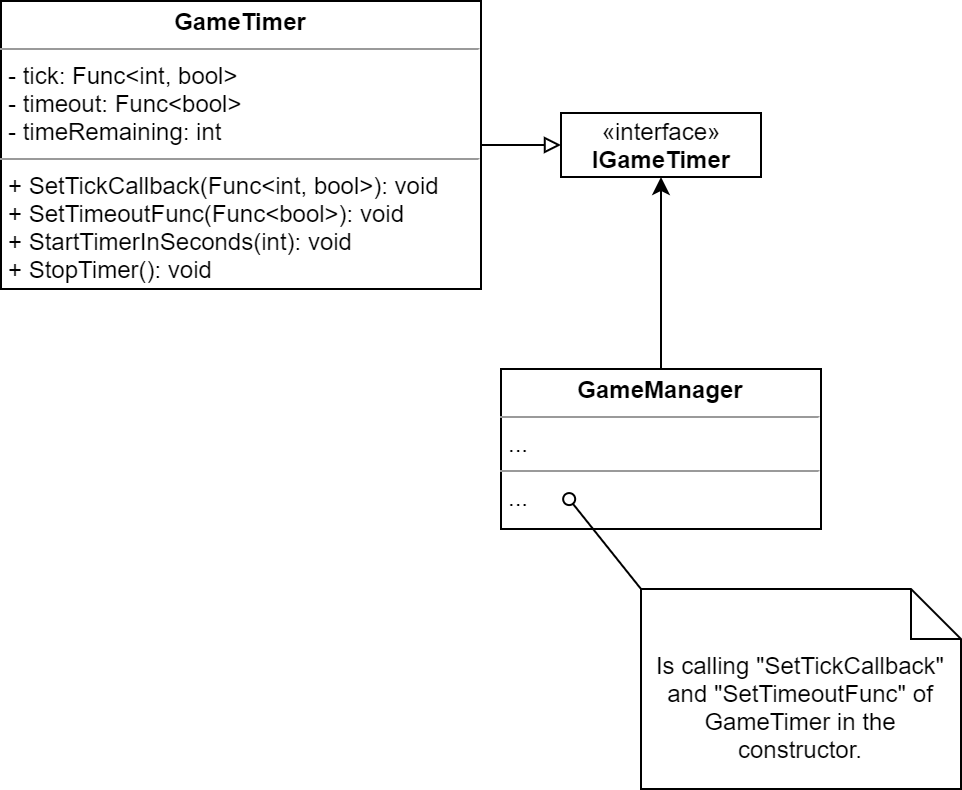
\includegraphics[width=0.7\textwidth]{Bilder/Entwurfsmuster.PNG}
\caption{\label{Abb:Entwurfsmuster}UML Diagramm des Beobachter Entwurfsmusters}
\end{figure}

\newpage
\paragraph{Abstrakte Fabrik}
Als zweites Entwurfsmuster wurde das Erzeugungsmuster der Abstrakten Fabrik verwendet. Dieses wurde während der Implementierung der Clean Architecture verwendet und bereits in Kapitel~\ref{cleanArchitecture} erläutert. Es wurde bspw. für die \href{https://github.com/EinToni/Wortfinder/blob/main/Wortfinder/WordGenerator.cs}{\textit{WordFinder}} Klasse in Commit \href{https://github.com/EinToni/Wortfinder/commit/586681478211a26abc661239ecc2c297ef77041e}{586681478211a26abc661239ecc2c297ef77041e} implementiert (vgl. Abbildung~\ref{Abb:AbstrakteFabrik}) und später aufgrund der beschriebenen Umstrukturierung wieder entfernt.

\paragraph{Singleton}
Als drittes Entwurfsmuster wurde die Abwesenheit des Erzeugungsmusters Singleton festgestellt. Von jeder Klasse können mehrere Instanzen erzeugt werden und eine Klasse welche bei einem Aufruf wie \glqq GetInstance()\grqq{} die (einzige) Instanz einer anderen Klasse zurück gibt, gibt es nicht.

\endinput
\chapter{Programming Principles}
\section{SOLID}
\paragraph{Single responsibility principle}
Die meisten Klassen in der Anwendung erfüllen das Prinzip. Eine Klasse welches es allerdings nicht erfüllt hat, ist der \textit{MainWindowController}. Dieser war zum einen der Adapter zwischen dem \textit{MainWindow} und dem \textit{GameManager} hat aber auch das verbinden von Buchstaben in der GUI kontrolliert. Die Funktionalitäten zum Verbinden von Buchstaben wurde daher in eine Neue Klasse \textit{WordBuilder} ausgelagert, Commit \href{https://github.com/EinToni/Wortfinder/commit/817e4b1b6be02defe58792a4afb709c7a147ced5}{817e4b1b6be02defe58792a4afb709c7a147ced5} und der darauf folgende. 


\paragraph{Open/Closed principle}
Eine auffällige Verbesserungsmöglichkeit wurde im \textit{GameScoreCalculator} gefunden, welcher immer wieder modifiziert wurde um die Punktzahl anders zu berechnen. Die Berechnung wurde nun Erweiterbar ausgelagert. Dafür wurde eine Liste im \textit{GameScoreCalculator} erstellt welche Klassen eines \textit{IPointFactor} Interfaces beinhaltet. Über diese wird beim Berechnen der Punkte Iteriert und jede Klasse berechnet dann einen Teilbetrag der Punktzahl, bezogen auf einen bestimmten Faktor. Siehe Commit \href{https://github.com/EinToni/Wortfinder/commit/6a4834cfc653a63ed3efc8745bccbe603250da74}{6a4834cfc653a63ed3efc8745bccbe603250da74}.


\paragraph{Liskov substitution principle}
Da keine Vererbung verwendet wird, ist das Liskov substitution principle erfüllt.

\paragraph{Dependency inversion principle}
Dependency inversion wurde im Rahmen der Implementierung der Clean Architecture an allen Grenzen der einzelnen Schichten angewendet.

\section{GRASP}
\paragraph{Grundkonzept} Der Code hat stellenweise eine recht hohe Kopplung, da oft Funktionen innerhalb der selben Klasse aufgerufen werden. Oftmals ist die Kopplung aber auch niedrig, weil für viele Klassen Interfaces verwendet und diese aufgerufen werden. Die Kohäsion ist vor allem im Domain und Application code recht hoch.


\paragraph{Code-Strukturierung}
Es wird viel Indirection verwendet. Ein gutes Beispiel dafür ist der \textit{GameManager}, welcher im Grunde alle aufrufe an verschiedene andere Klassen weiterleitet.


\paragraph{Architektur}
\glqq Pure fabrication\grqq{} findet sich in der \textit{EnDecoder} Klasse wieder. Diese ist unabhängig von jeglicher Anwendungslogik und ver- bzw. entschlüsselt einen beliebigen Stream mit einem beliebigen key in ein beliebiges Verzeichnis.


\paragraph{Entwurfsmuster}
Die GUI kommuniziert immer nur mit einen Controller. Ein Beispiel ist der \textit{MainWindowController}. Dieser Leitet die Aufrufe weiter und wandelt teilweise Datentypen um.


\section{DRY}
Das \glqq don't repeat yourself\grqq{} Prinzip wurde im Produktivcode meistens eingehalten, da die Informationen als Klassen Parameter gespeichert und wiederverwendet wurden. Somit ist die Information nur an einem Ort gespeichert. Innerhalb von Tests wurde das Prinzip allerdings häufig nicht eingehalten. Weil die Tests oft schnell geschrieben wurden, wurden meistens keine extra Variablen angelegt, sondern die Informationen mehrfach geschrieben. Die Anpassungen der Tests sind in Commit \href{https://github.com/EinToni/Wortfinder/commit/31e056a85512623173a8e4efa2faa828b2f66466}{31e056a85512623173a8e4efa2faa828b2f66466}.
\endinput

% Ab hier beginnt der Anhang
\appendix
\cleardoublepage
\pagenumbering{Roman}
\setcounter{page}{\thesavepage}
\addcontentsline{toc}{chapter}{Anhang}
\chapter{Abbildungen}

\begin{figure}[!ht]
  \centering
  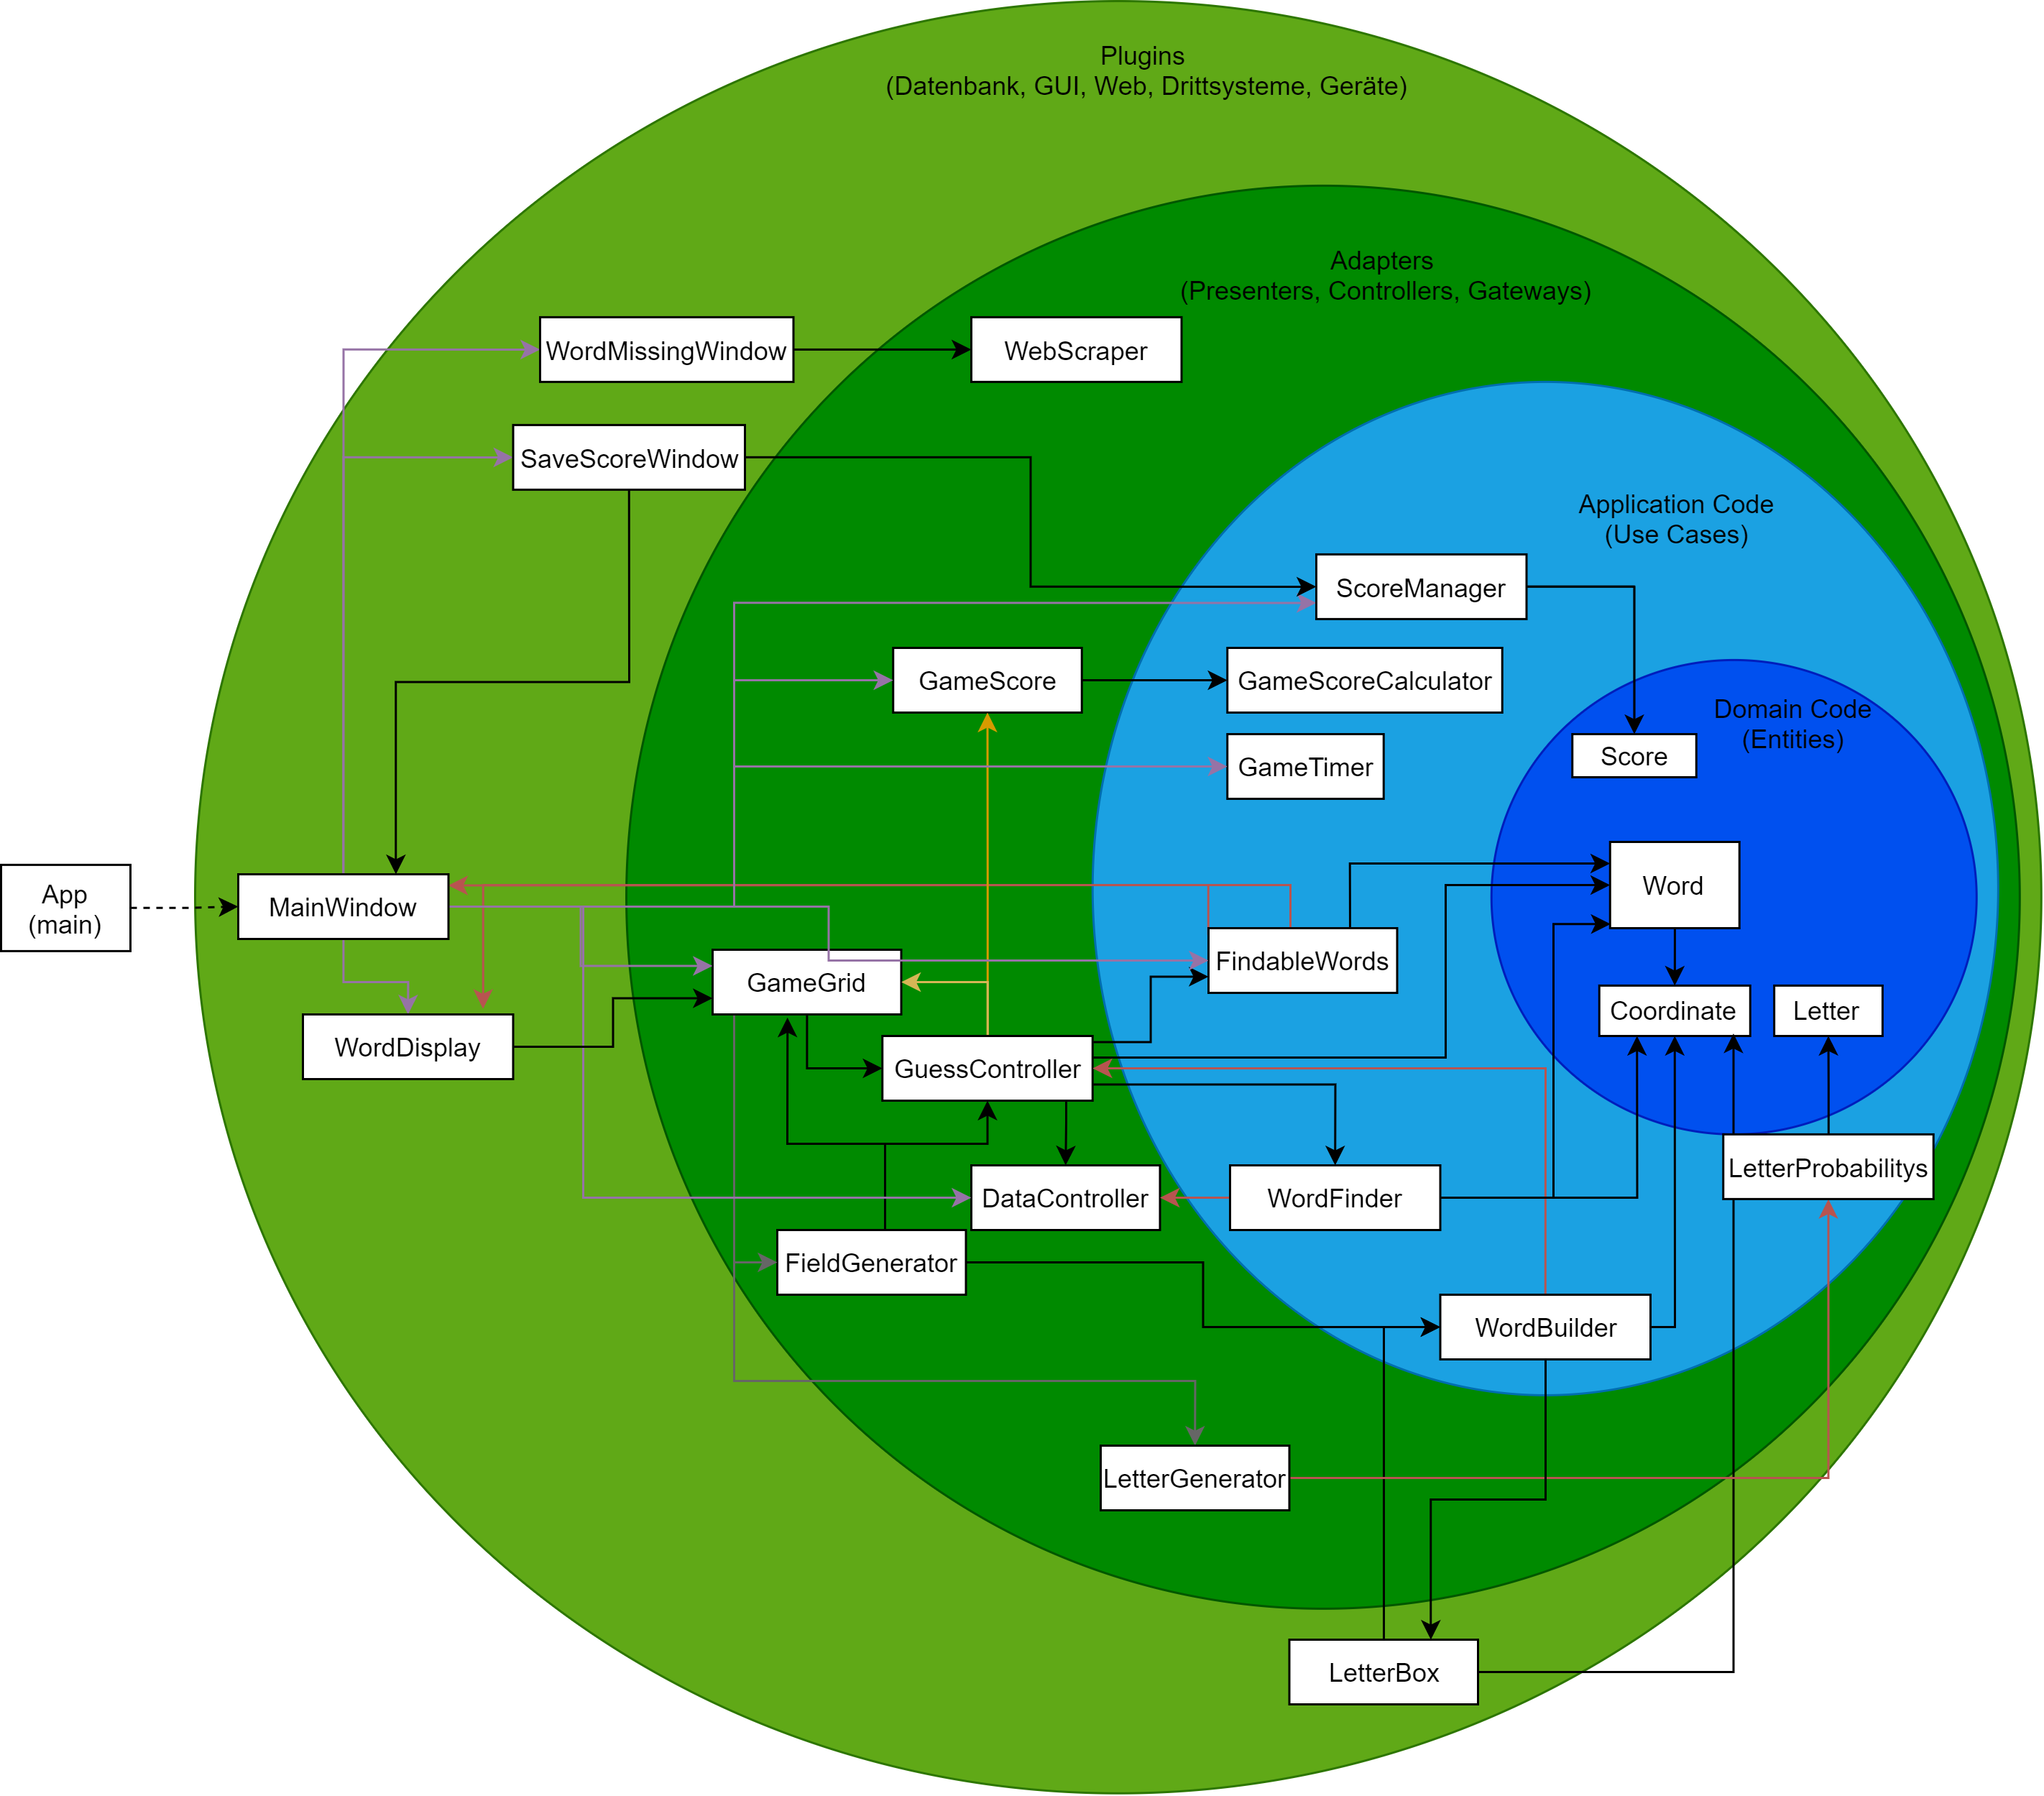
\includegraphics[width=0.9\textwidth]{Bilder/CleanArchitectureBEFORE.PNG}
  \caption[UML Klassendiagramm vor der Clean Architecture]{UML Klassendiagramm vor der Clean Architecture \href{https://github.com/EinToni/WortfinderDoku/blob/main/Bilder/CleanArchitectureBEFORE.png}{(link)}}
  \label{Abb:CleanArchitectureBEFORE}
\end{figure}

\begin{figure}[!ht]
  \centering
  \includegraphics[height=0.78\textheight, angle =90]{Bilder/CleanArchitectureAFTER.PNG}
  \caption[UML Diagramm nach der Clean Architecture]{UML Diagramm nach der Clean Architecture \href{https://github.com/EinToni/WortfinderDoku/blob/main/Bilder/CleanArchitectureAFTER.png}{(link)}}
  \label{Abb:CleanArchitectureAFTER}
\end{figure}

\begin{figure}[!ht]
  \centering
  \includegraphics[height=0.78\textheight, angle =90]{Bilder/CleanArchitectureAFTERinMain.PNG}
  \caption[UML Diagramm nach der Clean Architecture mit der Initialisierung in der Main]{UML Diagramm nach der Clean Architecture \href{https://github.com/EinToni/WortfinderDoku/blob/main/Bilder/CleanArchitectureAFTERinMain.png}{(link)}}
  \label{Abb:CleanArchitectureAFTERinMain}
\end{figure}

\endinput

\end{document}